\documentclass[twoside]{book}

% Packages required by doxygen
\usepackage{fixltx2e}
\usepackage{calc}
\usepackage{doxygen}
\usepackage[export]{adjustbox} % also loads graphicx
\usepackage{graphicx}
\usepackage[utf8]{inputenc}
\usepackage{makeidx}
\usepackage{multicol}
\usepackage{multirow}
\PassOptionsToPackage{warn}{textcomp}
\usepackage{textcomp}
\usepackage[nointegrals]{wasysym}
\usepackage[table]{xcolor}

% Font selection
\usepackage[T1]{fontenc}
\usepackage[scaled=.90]{helvet}
\usepackage{courier}
\usepackage{amssymb}
\usepackage{sectsty}
\renewcommand{\familydefault}{\sfdefault}
\allsectionsfont{%
  \fontseries{bc}\selectfont%
  \color{darkgray}%
}
\renewcommand{\DoxyLabelFont}{%
  \fontseries{bc}\selectfont%
  \color{darkgray}%
}
\newcommand{\+}{\discretionary{\mbox{\scriptsize$\hookleftarrow$}}{}{}}

% Page & text layout
\usepackage{geometry}
\geometry{%
  a4paper,%
  top=2.5cm,%
  bottom=2.5cm,%
  left=2.5cm,%
  right=2.5cm%
}
\tolerance=750
\hfuzz=15pt
\hbadness=750
\setlength{\emergencystretch}{15pt}
\setlength{\parindent}{0cm}
\setlength{\parskip}{3ex plus 2ex minus 2ex}
\makeatletter
\renewcommand{\paragraph}{%
  \@startsection{paragraph}{4}{0ex}{-1.0ex}{1.0ex}{%
    \normalfont\normalsize\bfseries\SS@parafont%
  }%
}
\renewcommand{\subparagraph}{%
  \@startsection{subparagraph}{5}{0ex}{-1.0ex}{1.0ex}{%
    \normalfont\normalsize\bfseries\SS@subparafont%
  }%
}
\makeatother

% Headers & footers
\usepackage{fancyhdr}
\pagestyle{fancyplain}
\fancyhead[LE]{\fancyplain{}{\bfseries\thepage}}
\fancyhead[CE]{\fancyplain{}{}}
\fancyhead[RE]{\fancyplain{}{\bfseries\leftmark}}
\fancyhead[LO]{\fancyplain{}{\bfseries\rightmark}}
\fancyhead[CO]{\fancyplain{}{}}
\fancyhead[RO]{\fancyplain{}{\bfseries\thepage}}
\fancyfoot[LE]{\fancyplain{}{}}
\fancyfoot[CE]{\fancyplain{}{}}
\fancyfoot[RE]{\fancyplain{}{\bfseries\scriptsize Generated by Doxygen }}
\fancyfoot[LO]{\fancyplain{}{\bfseries\scriptsize Generated by Doxygen }}
\fancyfoot[CO]{\fancyplain{}{}}
\fancyfoot[RO]{\fancyplain{}{}}
\renewcommand{\footrulewidth}{0.4pt}
\renewcommand{\chaptermark}[1]{%
  \markboth{#1}{}%
}
\renewcommand{\sectionmark}[1]{%
  \markright{\thesection\ #1}%
}

% Indices & bibliography
\usepackage{natbib}
\usepackage[titles]{tocloft}
\setcounter{tocdepth}{3}
\setcounter{secnumdepth}{5}
\makeindex

% Custom commands
\newcommand{\clearemptydoublepage}{%
  \newpage{\pagestyle{empty}\cleardoublepage}%
}

\usepackage{caption}
\captionsetup{labelsep=space,justification=centering,font={bf},singlelinecheck=off,skip=4pt,position=top}

%===== C O N T E N T S =====

\begin{document}

% Titlepage & ToC
\pagenumbering{roman}
\begin{titlepage}
\vspace*{7cm}
\begin{center}%
{\Large lab2 }\\
\vspace*{1cm}
{\large Generated by Doxygen 1.8.11}\\
\end{center}
\end{titlepage}
\clearemptydoublepage
\tableofcontents
\clearemptydoublepage
\pagenumbering{arabic}

%--- Begin generated contents ---
\chapter{Hierarchical Index}
\section{Class Hierarchy}
This inheritance list is sorted roughly, but not completely, alphabetically\+:\begin{DoxyCompactList}
\item \contentsline{section}{General\+Number}{\pageref{classGeneralNumber}}{}
\begin{DoxyCompactList}
\item \contentsline{section}{General\+Long}{\pageref{classGeneralLong}}{}
\item \contentsline{section}{General\+Rational}{\pageref{classGeneralRational}}{}
\end{DoxyCompactList}
\end{DoxyCompactList}

\chapter{Class Index}
\section{Class List}
Here are the classes, structs, unions and interfaces with brief descriptions\+:\begin{DoxyCompactList}
\item\contentsline{section}{{\bf General\+Long} }{\pageref{classGeneralLong}}{}
\item\contentsline{section}{{\bf General\+Number} }{\pageref{classGeneralNumber}}{}
\item\contentsline{section}{{\bf General\+Rational} }{\pageref{classGeneralRational}}{}
\end{DoxyCompactList}

\chapter{File Index}
\section{File List}
Here is a list of all files with brief descriptions\+:\begin{DoxyCompactList}
\item\contentsline{section}{{\bf General\+Number.\+cpp} }{\pageref{GeneralNumber_8cpp}}{}
\item\contentsline{section}{{\bf General\+Number.\+h} }{\pageref{GeneralNumber_8h}}{}
\item\contentsline{section}{{\bf gntest.\+cpp} }{\pageref{gntest_8cpp}}{}
\end{DoxyCompactList}

\chapter{Class Documentation}
\section{General\+Long Class Reference}
\label{classGeneralLong}\index{General\+Long@{General\+Long}}


{\ttfamily \#include $<$General\+Number.\+h$>$}

Inheritance diagram for General\+Long\+:\begin{figure}[H]
\begin{center}
\leavevmode
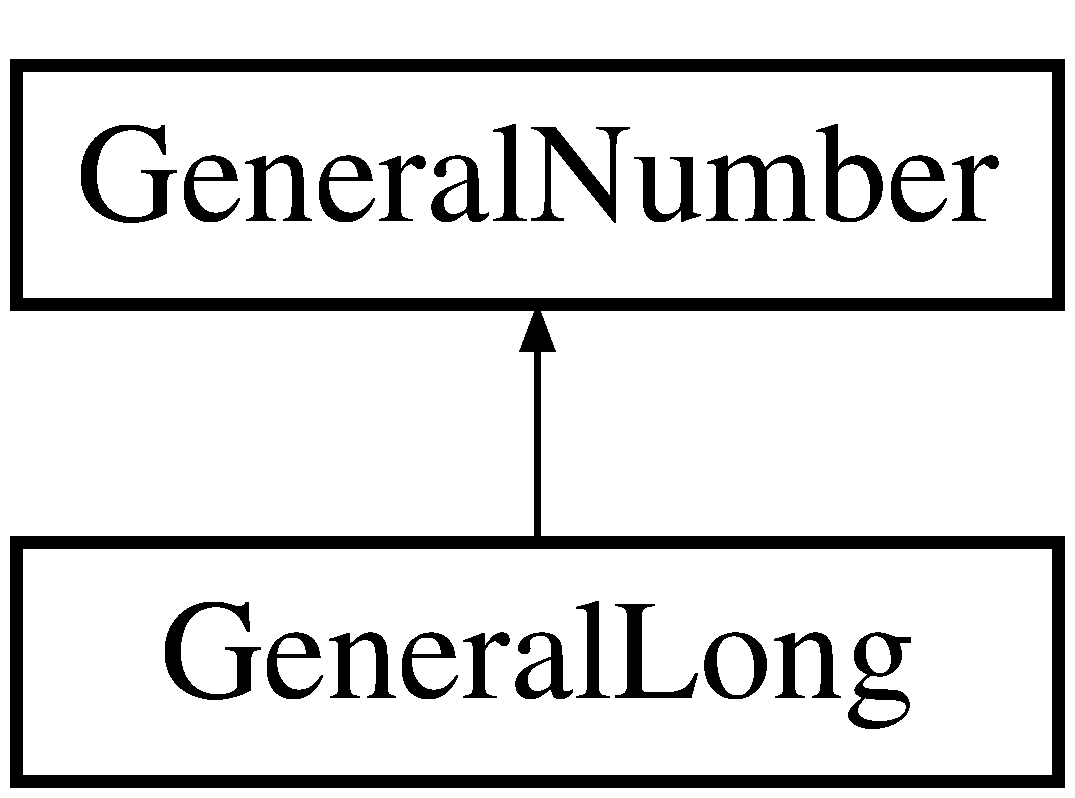
\includegraphics[height=2.000000cm]{classGeneralLong}
\end{center}
\end{figure}
\subsection*{Public Member Functions}
\begin{DoxyCompactItemize}
\item 
{\bf General\+Long} ()
\item 
{\bf General\+Long} (long {\bf value})
\item 
char $\ast$ {\bf to\+String} () const 
\item 
char $\ast$ {\bf foo} () const 
\item 
{\bf General\+Long} $\ast$ {\bf to\+General\+Long} () const 
\item 
{\bf General\+Rational} $\ast$ {\bf to\+General\+Rational} () const 
\item 
long {\bf get\+Value} ()
\item 
{\bf General\+Number} $\ast$ {\bf sum\+With} ({\bf General\+Number} $\ast$num)
\end{DoxyCompactItemize}
\subsection*{Private Attributes}
\begin{DoxyCompactItemize}
\item 
long {\bf value}
\end{DoxyCompactItemize}


\subsection{Constructor \& Destructor Documentation}
\index{General\+Long@{General\+Long}!General\+Long@{General\+Long}}
\index{General\+Long@{General\+Long}!General\+Long@{General\+Long}}
\subsubsection[{General\+Long()}]{\setlength{\rightskip}{0pt plus 5cm}General\+Long\+::\+General\+Long (
\begin{DoxyParamCaption}
{}
\end{DoxyParamCaption}
)}\label{classGeneralLong_a9ba8d9844c5826284493301e3834e0fa}
Default constructor for \doxyref{General\+Long}{p.}{classGeneralLong} \index{General\+Long@{General\+Long}!General\+Long@{General\+Long}}
\index{General\+Long@{General\+Long}!General\+Long@{General\+Long}}
\subsubsection[{General\+Long(long value)}]{\setlength{\rightskip}{0pt plus 5cm}General\+Long\+::\+General\+Long (
\begin{DoxyParamCaption}
\item[{long}]{value}
\end{DoxyParamCaption}
)}\label{classGeneralLong_ac76419bcc51c55390d4b886f4c1ea828}
Constructor for \doxyref{General\+Long}{p.}{classGeneralLong} 
\begin{DoxyParams}{Parameters}
{\em value} & Number to store in the object \\
\hline
\end{DoxyParams}


\subsection{Member Function Documentation}
\index{General\+Long@{General\+Long}!foo@{foo}}
\index{foo@{foo}!General\+Long@{General\+Long}}
\subsubsection[{foo() const }]{\setlength{\rightskip}{0pt plus 5cm}char $\ast$ General\+Long\+::foo (
\begin{DoxyParamCaption}
{}
\end{DoxyParamCaption}
) const}\label{classGeneralLong_a9c7e995eb89b06f3db51c0b5faaa272c}
Demonstrates a non-\/virtual function. \begin{DoxyReturn}{Returns}
Freshly-\/allocated C-\/stype string 
\end{DoxyReturn}


Referenced by main().

\index{General\+Long@{General\+Long}!get\+Value@{get\+Value}}
\index{get\+Value@{get\+Value}!General\+Long@{General\+Long}}
\subsubsection[{get\+Value()}]{\setlength{\rightskip}{0pt plus 5cm}long General\+Long\+::get\+Value (
\begin{DoxyParamCaption}
{}
\end{DoxyParamCaption}
)}\label{classGeneralLong_af25d9a4f795b2046b3d0fb147b588101}
Gets the value of this general long

\begin{DoxyReturn}{Returns}
value of general long 
\end{DoxyReturn}


Referenced by sum\+With().

\index{General\+Long@{General\+Long}!sum\+With@{sum\+With}}
\index{sum\+With@{sum\+With}!General\+Long@{General\+Long}}
\subsubsection[{sum\+With(\+General\+Number $\ast$num)}]{\setlength{\rightskip}{0pt plus 5cm}{\bf General\+Number} $\ast$ General\+Long\+::sum\+With (
\begin{DoxyParamCaption}
\item[{{\bf General\+Number} $\ast$}]{num}
\end{DoxyParamCaption}
)\hspace{0.3cm}{\ttfamily [virtual]}}\label{classGeneralLong_a1f079c0275301d4fd4332d481cc5787f}
Sums two numbers of type \doxyref{General\+Number}{p.}{classGeneralNumber} together


\begin{DoxyParams}{Parameters}
{\em num} & pointer to \doxyref{General\+Number}{p.}{classGeneralNumber} \\
\hline
\end{DoxyParams}
\begin{DoxyReturn}{Returns}
\doxyref{General\+Long}{p.}{classGeneralLong} holding resutls of summation 
\end{DoxyReturn}


Reimplemented from {\bf General\+Number} \doxyref{}{p.}{classGeneralNumber_ab40df9cc601a20e8f08d7c2c50e0875e}.



References get\+Value(), and General\+Number\+::to\+General\+Long().



Referenced by main().

\index{General\+Long@{General\+Long}!to\+General\+Long@{to\+General\+Long}}
\index{to\+General\+Long@{to\+General\+Long}!General\+Long@{General\+Long}}
\subsubsection[{to\+General\+Long() const }]{\setlength{\rightskip}{0pt plus 5cm}{\bf General\+Long} $\ast$ General\+Long\+::to\+General\+Long (
\begin{DoxyParamCaption}
{}
\end{DoxyParamCaption}
) const\hspace{0.3cm}{\ttfamily [virtual]}}\label{classGeneralLong_a67fdd908d3af4a8fefc0657f2eb86dd0}
Generates an equivalent \doxyref{General\+Long}{p.}{classGeneralLong} \begin{DoxyReturn}{Returns}
Pointer to a freshly-\/allocated \doxyref{General\+Long}{p.}{classGeneralLong} object 
\end{DoxyReturn}


Reimplemented from {\bf General\+Number} \doxyref{}{p.}{classGeneralNumber_a3257176764dd42f884f3d32bc26cd508}.

\index{General\+Long@{General\+Long}!to\+General\+Rational@{to\+General\+Rational}}
\index{to\+General\+Rational@{to\+General\+Rational}!General\+Long@{General\+Long}}
\subsubsection[{to\+General\+Rational() const }]{\setlength{\rightskip}{0pt plus 5cm}{\bf General\+Rational} $\ast$ General\+Long\+::to\+General\+Rational (
\begin{DoxyParamCaption}
{}
\end{DoxyParamCaption}
) const\hspace{0.3cm}{\ttfamily [virtual]}}\label{classGeneralLong_aa983396c8843991c6bbea52b1d22e51b}
Generates an equivalent \doxyref{General\+Rational}{p.}{classGeneralRational} \begin{DoxyReturn}{Returns}
Pointer to a freshly-\/allocated \doxyref{General\+Rational}{p.}{classGeneralRational} object 
\end{DoxyReturn}


Reimplemented from {\bf General\+Number} \doxyref{}{p.}{classGeneralNumber_ae92a1bfb38c40bcda30fd93335a4ea54}.



Referenced by main().

\index{General\+Long@{General\+Long}!to\+String@{to\+String}}
\index{to\+String@{to\+String}!General\+Long@{General\+Long}}
\subsubsection[{to\+String() const }]{\setlength{\rightskip}{0pt plus 5cm}char $\ast$ General\+Long\+::to\+String (
\begin{DoxyParamCaption}
{}
\end{DoxyParamCaption}
) const\hspace{0.3cm}{\ttfamily [virtual]}}\label{classGeneralLong_ae3afbc099d82bf5a8eb7d8e9ac32cb87}
Generates a printable representation of the object. \begin{DoxyReturn}{Returns}
Freshly-\/allocated C-\/stype string 
\end{DoxyReturn}


Reimplemented from {\bf General\+Number} \doxyref{}{p.}{classGeneralNumber_a071819b67064dc17754ff7cdc4964d75}.



References M\+A\+X\+\_\+\+D\+I\+G\+I\+T\+S\+\_\+\+I\+N\+\_\+\+L\+O\+NG.



Referenced by main().



\subsection{Member Data Documentation}
\index{General\+Long@{General\+Long}!value@{value}}
\index{value@{value}!General\+Long@{General\+Long}}
\subsubsection[{value}]{\setlength{\rightskip}{0pt plus 5cm}long General\+Long\+::value\hspace{0.3cm}{\ttfamily [private]}}\label{classGeneralLong_a3a25ceb37f06367fd5cf2b22e97289aa}


The documentation for this class was generated from the following files\+:\begin{DoxyCompactItemize}
\item 
{\bf General\+Number.\+h}\item 
{\bf General\+Number.\+cpp}\end{DoxyCompactItemize}

\section{General\+Number Class Reference}
\label{classGeneralNumber}\index{General\+Number@{General\+Number}}


{\ttfamily \#include $<$General\+Number.\+h$>$}

Inheritance diagram for General\+Number\+:\begin{figure}[H]
\begin{center}
\leavevmode
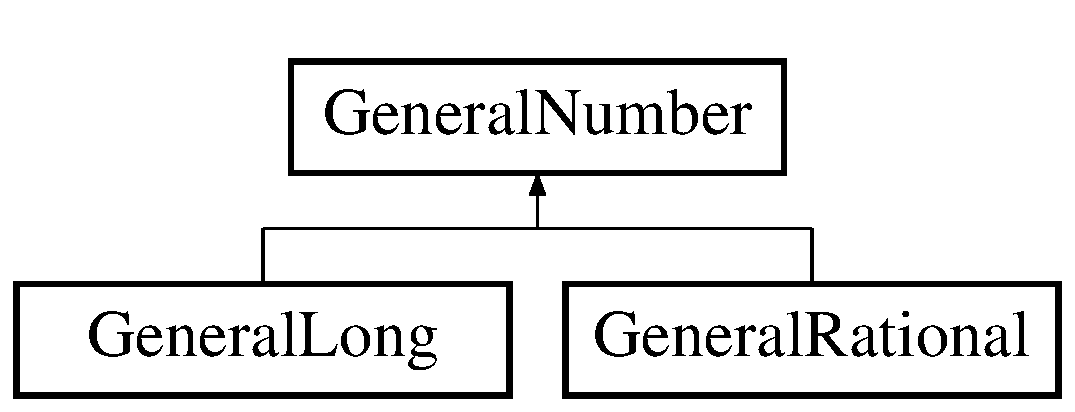
\includegraphics[height=2.000000cm]{classGeneralNumber}
\end{center}
\end{figure}
\subsection*{Public Member Functions}
\begin{DoxyCompactItemize}
\item 
{\bf General\+Number} ()
\item 
virtual char $\ast$ {\bf to\+String} () const 
\item 
char $\ast$ {\bf foo} () const 
\item 
virtual {\bf General\+Long} $\ast$ {\bf to\+General\+Long} () const 
\item 
virtual {\bf General\+Rational} $\ast$ {\bf to\+General\+Rational} () const 
\item 
virtual {\bf General\+Number} $\ast$ {\bf sum\+With} ({\bf General\+Number} $\ast$num)
\end{DoxyCompactItemize}


\subsection{Constructor \& Destructor Documentation}
\index{General\+Number@{General\+Number}!General\+Number@{General\+Number}}
\index{General\+Number@{General\+Number}!General\+Number@{General\+Number}}
\subsubsection[{General\+Number()}]{\setlength{\rightskip}{0pt plus 5cm}General\+Number\+::\+General\+Number (
\begin{DoxyParamCaption}
{}
\end{DoxyParamCaption}
)}\label{classGeneralNumber_a3c08bdccb4a03c82932546d5c19e636d}
Default constructor for \doxyref{General\+Number}{p.}{classGeneralNumber} 

Referenced by sum\+With().



\subsection{Member Function Documentation}
\index{General\+Number@{General\+Number}!foo@{foo}}
\index{foo@{foo}!General\+Number@{General\+Number}}
\subsubsection[{foo() const }]{\setlength{\rightskip}{0pt plus 5cm}char $\ast$ General\+Number\+::foo (
\begin{DoxyParamCaption}
{}
\end{DoxyParamCaption}
) const}\label{classGeneralNumber_afedc95deda6c653dd57485930865b6ca}
Demonstrates a non-\/virtual function. \begin{DoxyReturn}{Returns}
Freshly-\/allocated C-\/stype string 
\end{DoxyReturn}


Referenced by main().

\index{General\+Number@{General\+Number}!sum\+With@{sum\+With}}
\index{sum\+With@{sum\+With}!General\+Number@{General\+Number}}
\subsubsection[{sum\+With(\+General\+Number $\ast$num)}]{\setlength{\rightskip}{0pt plus 5cm}{\bf General\+Number} $\ast$ General\+Number\+::sum\+With (
\begin{DoxyParamCaption}
\item[{{\bf General\+Number} $\ast$}]{num}
\end{DoxyParamCaption}
)\hspace{0.3cm}{\ttfamily [virtual]}}\label{classGeneralNumber_ab40df9cc601a20e8f08d7c2c50e0875e}
Default sum\+With function. Just returns empty \doxyref{General\+Number}{p.}{classGeneralNumber} when called in the \doxyref{General\+Number}{p.}{classGeneralNumber} class


\begin{DoxyParams}{Parameters}
{\em General\+Number$\ast$} & number to sum \\
\hline
\end{DoxyParams}
\begin{DoxyReturn}{Returns}
Empty \doxyref{General\+Number}{p.}{classGeneralNumber} 
\end{DoxyReturn}


Reimplemented in {\bf General\+Rational} \doxyref{}{p.}{classGeneralRational_a993edff04590c7e9409e7e4f92a3e8b6}, and {\bf General\+Long} \doxyref{}{p.}{classGeneralLong_a1f079c0275301d4fd4332d481cc5787f}.



References General\+Number().

\index{General\+Number@{General\+Number}!to\+General\+Long@{to\+General\+Long}}
\index{to\+General\+Long@{to\+General\+Long}!General\+Number@{General\+Number}}
\subsubsection[{to\+General\+Long() const }]{\setlength{\rightskip}{0pt plus 5cm}{\bf General\+Long} $\ast$ General\+Number\+::to\+General\+Long (
\begin{DoxyParamCaption}
{}
\end{DoxyParamCaption}
) const\hspace{0.3cm}{\ttfamily [virtual]}}\label{classGeneralNumber_a3257176764dd42f884f3d32bc26cd508}
Generates an equivalent \doxyref{General\+Long}{p.}{classGeneralLong} \begin{DoxyReturn}{Returns}
Pointer to a freshly-\/allocated \doxyref{General\+Long}{p.}{classGeneralLong} object 
\end{DoxyReturn}


Reimplemented in {\bf General\+Rational} \doxyref{}{p.}{classGeneralRational_aadd587b17b9ce5bc6beea2bf065e68ca}, and {\bf General\+Long} \doxyref{}{p.}{classGeneralLong_a67fdd908d3af4a8fefc0657f2eb86dd0}.



Referenced by main(), and General\+Long\+::sum\+With().

\index{General\+Number@{General\+Number}!to\+General\+Rational@{to\+General\+Rational}}
\index{to\+General\+Rational@{to\+General\+Rational}!General\+Number@{General\+Number}}
\subsubsection[{to\+General\+Rational() const }]{\setlength{\rightskip}{0pt plus 5cm}{\bf General\+Rational} $\ast$ General\+Number\+::to\+General\+Rational (
\begin{DoxyParamCaption}
{}
\end{DoxyParamCaption}
) const\hspace{0.3cm}{\ttfamily [virtual]}}\label{classGeneralNumber_ae92a1bfb38c40bcda30fd93335a4ea54}
Generates an equivalent \doxyref{General\+Rational}{p.}{classGeneralRational} \begin{DoxyReturn}{Returns}
Pointer to a freshly-\/allocated \doxyref{General\+Rational}{p.}{classGeneralRational} object 
\end{DoxyReturn}


Reimplemented in {\bf General\+Rational} \doxyref{}{p.}{classGeneralRational_af474c9b5f3f31934c24ba47230cd5537}, and {\bf General\+Long} \doxyref{}{p.}{classGeneralLong_aa983396c8843991c6bbea52b1d22e51b}.



Referenced by General\+Rational\+::sum\+With().

\index{General\+Number@{General\+Number}!to\+String@{to\+String}}
\index{to\+String@{to\+String}!General\+Number@{General\+Number}}
\subsubsection[{to\+String() const }]{\setlength{\rightskip}{0pt plus 5cm}char $\ast$ General\+Number\+::to\+String (
\begin{DoxyParamCaption}
{}
\end{DoxyParamCaption}
) const\hspace{0.3cm}{\ttfamily [virtual]}}\label{classGeneralNumber_a071819b67064dc17754ff7cdc4964d75}
Generates a printable representation of the object. \begin{DoxyReturn}{Returns}
Freshly-\/allocated C-\/stype string 
\end{DoxyReturn}


Reimplemented in {\bf General\+Rational} \doxyref{}{p.}{classGeneralRational_a592adc36a0593c960c197741ab5b50b9}, and {\bf General\+Long} \doxyref{}{p.}{classGeneralLong_ae3afbc099d82bf5a8eb7d8e9ac32cb87}.



Referenced by main().



The documentation for this class was generated from the following files\+:\begin{DoxyCompactItemize}
\item 
{\bf General\+Number.\+h}\item 
{\bf General\+Number.\+cpp}\end{DoxyCompactItemize}

\section{General\+Rational Class Reference}
\label{classGeneralRational}\index{General\+Rational@{General\+Rational}}


{\ttfamily \#include $<$General\+Number.\+h$>$}

Inheritance diagram for General\+Rational\+:\begin{figure}[H]
\begin{center}
\leavevmode
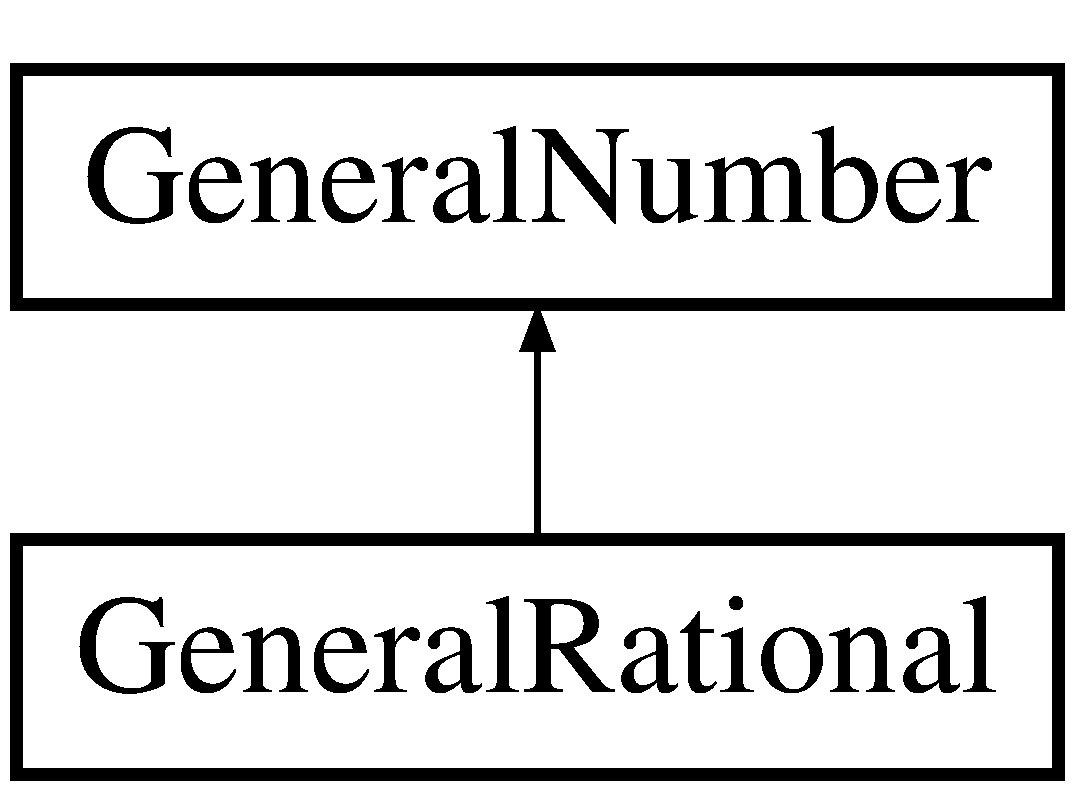
\includegraphics[height=2.000000cm]{classGeneralRational}
\end{center}
\end{figure}
\subsection*{Public Member Functions}
\begin{DoxyCompactItemize}
\item 
{\bf General\+Rational} ()
\item 
{\bf General\+Rational} (long {\bf top}, long {\bf bottom})
\item 
char $\ast$ {\bf to\+String} () const 
\item 
char $\ast$ {\bf foo} () const 
\item 
{\bf General\+Long} $\ast$ {\bf to\+General\+Long} () const 
\item 
{\bf General\+Rational} $\ast$ {\bf to\+General\+Rational} () const 
\item 
void {\bf canonicalize} ()
\item 
long {\bf get\+Top} ()
\item 
long {\bf get\+Bottom} ()
\item 
{\bf General\+Number} $\ast$ {\bf sum\+With} ({\bf General\+Number} $\ast$num)
\end{DoxyCompactItemize}
\subsection*{Private Attributes}
\begin{DoxyCompactItemize}
\item 
long {\bf top}
\item 
long {\bf bottom}
\end{DoxyCompactItemize}


\subsection{Constructor \& Destructor Documentation}
\index{General\+Rational@{General\+Rational}!General\+Rational@{General\+Rational}}
\index{General\+Rational@{General\+Rational}!General\+Rational@{General\+Rational}}
\subsubsection[{General\+Rational()}]{\setlength{\rightskip}{0pt plus 5cm}General\+Rational\+::\+General\+Rational (
\begin{DoxyParamCaption}
{}
\end{DoxyParamCaption}
)}\label{classGeneralRational_a681f589c9e7699dbb1fdafd136abf325}
Default constructor for \doxyref{General\+Rational}{p.}{classGeneralRational} \index{General\+Rational@{General\+Rational}!General\+Rational@{General\+Rational}}
\index{General\+Rational@{General\+Rational}!General\+Rational@{General\+Rational}}
\subsubsection[{General\+Rational(long top, long bottom)}]{\setlength{\rightskip}{0pt plus 5cm}General\+Rational\+::\+General\+Rational (
\begin{DoxyParamCaption}
\item[{long}]{top, }
\item[{long}]{bottom}
\end{DoxyParamCaption}
)}\label{classGeneralRational_aa6f7a00036226fa620d77ac1a345fae0}
Constructor for \doxyref{General\+Rational}{p.}{classGeneralRational} 
\begin{DoxyParams}{Parameters}
{\em top} & Numerator to store in the object \\
\hline
{\em bottom} & Denominator to store in the object \\
\hline
\end{DoxyParams}


\subsection{Member Function Documentation}
\index{General\+Rational@{General\+Rational}!canonicalize@{canonicalize}}
\index{canonicalize@{canonicalize}!General\+Rational@{General\+Rational}}
\subsubsection[{canonicalize()}]{\setlength{\rightskip}{0pt plus 5cm}void General\+Rational\+::canonicalize (
\begin{DoxyParamCaption}
{}
\end{DoxyParamCaption}
)}\label{classGeneralRational_a5fa2dde868fbca3a8edc03af0430c7db}
Canonicalizes a \doxyref{General\+Rational}{p.}{classGeneralRational} Converts the \doxyref{General\+Rational}{p.}{classGeneralRational} to its canonical form. That is, the rational number is written in its simplest form. If the ratio is negative, the sign is on the numerator, and the denominator is positive. 

References G\+C\+D().



Referenced by main(), and sum\+With().

\index{General\+Rational@{General\+Rational}!foo@{foo}}
\index{foo@{foo}!General\+Rational@{General\+Rational}}
\subsubsection[{foo() const }]{\setlength{\rightskip}{0pt plus 5cm}char $\ast$ General\+Rational\+::foo (
\begin{DoxyParamCaption}
{}
\end{DoxyParamCaption}
) const}\label{classGeneralRational_a265451cfed295bc3711cf532ffa28d03}
Demonstrates a non-\/virtual function. \begin{DoxyReturn}{Returns}
Freshly-\/allocated C-\/stype string 
\end{DoxyReturn}
\index{General\+Rational@{General\+Rational}!get\+Bottom@{get\+Bottom}}
\index{get\+Bottom@{get\+Bottom}!General\+Rational@{General\+Rational}}
\subsubsection[{get\+Bottom()}]{\setlength{\rightskip}{0pt plus 5cm}long General\+Rational\+::get\+Bottom (
\begin{DoxyParamCaption}
{}
\end{DoxyParamCaption}
)}\label{classGeneralRational_a1cedaf10de47bb62e010bee4734c8e33}
Returns denominator of rational

\begin{DoxyReturn}{Returns}
Denominator of this general rational 
\end{DoxyReturn}


Referenced by sum\+With().

\index{General\+Rational@{General\+Rational}!get\+Top@{get\+Top}}
\index{get\+Top@{get\+Top}!General\+Rational@{General\+Rational}}
\subsubsection[{get\+Top()}]{\setlength{\rightskip}{0pt plus 5cm}long General\+Rational\+::get\+Top (
\begin{DoxyParamCaption}
{}
\end{DoxyParamCaption}
)}\label{classGeneralRational_a35d6306b54c8382f1ee2921b205ca9d9}
Returns numerator of rational

\begin{DoxyReturn}{Returns}
Numerator of this general rational 
\end{DoxyReturn}


Referenced by sum\+With().

\index{General\+Rational@{General\+Rational}!sum\+With@{sum\+With}}
\index{sum\+With@{sum\+With}!General\+Rational@{General\+Rational}}
\subsubsection[{sum\+With(\+General\+Number $\ast$num)}]{\setlength{\rightskip}{0pt plus 5cm}{\bf General\+Number} $\ast$ General\+Rational\+::sum\+With (
\begin{DoxyParamCaption}
\item[{{\bf General\+Number} $\ast$}]{num\+Input}
\end{DoxyParamCaption}
)\hspace{0.3cm}{\ttfamily [virtual]}}\label{classGeneralRational_a993edff04590c7e9409e7e4f92a3e8b6}
Sums this \doxyref{General\+Rational}{p.}{classGeneralRational} with any \doxyref{General\+Number}{p.}{classGeneralNumber}


\begin{DoxyParams}{Parameters}
{\em num\+Input} & The General Number to sum with \\
\hline
\end{DoxyParams}
\begin{DoxyReturn}{Returns}
A \doxyref{General\+Rational}{p.}{classGeneralRational} summed with this and the input 
\end{DoxyReturn}


Reimplemented from {\bf General\+Number} \doxyref{}{p.}{classGeneralNumber_ab40df9cc601a20e8f08d7c2c50e0875e}.



References canonicalize(), G\+C\+D(), get\+Bottom(), get\+Top(), and General\+Number\+::to\+General\+Rational().



Referenced by main().

\index{General\+Rational@{General\+Rational}!to\+General\+Long@{to\+General\+Long}}
\index{to\+General\+Long@{to\+General\+Long}!General\+Rational@{General\+Rational}}
\subsubsection[{to\+General\+Long() const }]{\setlength{\rightskip}{0pt plus 5cm}{\bf General\+Long} $\ast$ General\+Rational\+::to\+General\+Long (
\begin{DoxyParamCaption}
{}
\end{DoxyParamCaption}
) const\hspace{0.3cm}{\ttfamily [virtual]}}\label{classGeneralRational_aadd587b17b9ce5bc6beea2bf065e68ca}
Generates an equivalent \doxyref{General\+Long}{p.}{classGeneralLong} \begin{DoxyReturn}{Returns}
Pointer to a freshly-\/allocated \doxyref{General\+Long}{p.}{classGeneralLong} object 
\end{DoxyReturn}


Reimplemented from {\bf General\+Number} \doxyref{}{p.}{classGeneralNumber_a3257176764dd42f884f3d32bc26cd508}.

\index{General\+Rational@{General\+Rational}!to\+General\+Rational@{to\+General\+Rational}}
\index{to\+General\+Rational@{to\+General\+Rational}!General\+Rational@{General\+Rational}}
\subsubsection[{to\+General\+Rational() const }]{\setlength{\rightskip}{0pt plus 5cm}{\bf General\+Rational} $\ast$ General\+Rational\+::to\+General\+Rational (
\begin{DoxyParamCaption}
{}
\end{DoxyParamCaption}
) const\hspace{0.3cm}{\ttfamily [virtual]}}\label{classGeneralRational_af474c9b5f3f31934c24ba47230cd5537}
Generates an equivalent \doxyref{General\+Rational}{p.}{classGeneralRational} \begin{DoxyReturn}{Returns}
Pointer to a freshly-\/allocated \doxyref{General\+Rational}{p.}{classGeneralRational} object 
\end{DoxyReturn}


Reimplemented from {\bf General\+Number} \doxyref{}{p.}{classGeneralNumber_ae92a1bfb38c40bcda30fd93335a4ea54}.

\index{General\+Rational@{General\+Rational}!to\+String@{to\+String}}
\index{to\+String@{to\+String}!General\+Rational@{General\+Rational}}
\subsubsection[{to\+String() const }]{\setlength{\rightskip}{0pt plus 5cm}char $\ast$ General\+Rational\+::to\+String (
\begin{DoxyParamCaption}
{}
\end{DoxyParamCaption}
) const\hspace{0.3cm}{\ttfamily [virtual]}}\label{classGeneralRational_a592adc36a0593c960c197741ab5b50b9}
Generates a printable representation of the object. \begin{DoxyReturn}{Returns}
Freshly-\/allocated C-\/stype string 
\end{DoxyReturn}


Reimplemented from {\bf General\+Number} \doxyref{}{p.}{classGeneralNumber_a071819b67064dc17754ff7cdc4964d75}.



References M\+A\+X\+\_\+\+D\+I\+G\+I\+T\+S\+\_\+\+I\+N\+\_\+\+L\+O\+NG.



Referenced by main().



\subsection{Member Data Documentation}
\index{General\+Rational@{General\+Rational}!bottom@{bottom}}
\index{bottom@{bottom}!General\+Rational@{General\+Rational}}
\subsubsection[{bottom}]{\setlength{\rightskip}{0pt plus 5cm}long General\+Rational\+::bottom\hspace{0.3cm}{\ttfamily [private]}}\label{classGeneralRational_a74835ffcc9a7b1026658da2fb75dc0d7}
\index{General\+Rational@{General\+Rational}!top@{top}}
\index{top@{top}!General\+Rational@{General\+Rational}}
\subsubsection[{top}]{\setlength{\rightskip}{0pt plus 5cm}long General\+Rational\+::top\hspace{0.3cm}{\ttfamily [private]}}\label{classGeneralRational_a771617023f9c874e6920b001ab394a57}


The documentation for this class was generated from the following files\+:\begin{DoxyCompactItemize}
\item 
{\bf General\+Number.\+h}\item 
{\bf General\+Number.\+cpp}\end{DoxyCompactItemize}

\chapter{File Documentation}
\section{General\+Number.\+cpp File Reference}
\label{GeneralNumber_8cpp}\index{General\+Number.\+cpp@{General\+Number.\+cpp}}
{\ttfamily \#include $<$stdio.\+h$>$}\\*
{\ttfamily \#include $<$string.\+h$>$}\\*
{\ttfamily \#include $<$stdlib.\+h$>$}\\*
{\ttfamily \#include \char`\"{}General\+Number.\+h\char`\"{}}\\*
\subsection*{Functions}
\begin{DoxyCompactItemize}
\item 
long {\bf gcd\+\_\+\+Helper} (long A, long B)
\item 
long {\bf G\+CD} (long A, long B)
\end{DoxyCompactItemize}


\subsection{Function Documentation}
\index{General\+Number.\+cpp@{General\+Number.\+cpp}!G\+CD@{G\+CD}}
\index{G\+CD@{G\+CD}!General\+Number.\+cpp@{General\+Number.\+cpp}}
\subsubsection[{G\+C\+D(long A, long B)}]{\setlength{\rightskip}{0pt plus 5cm}long G\+CD (
\begin{DoxyParamCaption}
\item[{long}]{A, }
\item[{long}]{B}
\end{DoxyParamCaption}
)}\label{GeneralNumber_8cpp_a497677c0cabda13df5d6b8abbad9e1af}


References gcd\+\_\+\+Helper().



Referenced by General\+Rational\+::canonicalize(), and General\+Rational\+::sum\+With().

\index{General\+Number.\+cpp@{General\+Number.\+cpp}!gcd\+\_\+\+Helper@{gcd\+\_\+\+Helper}}
\index{gcd\+\_\+\+Helper@{gcd\+\_\+\+Helper}!General\+Number.\+cpp@{General\+Number.\+cpp}}
\subsubsection[{gcd\+\_\+\+Helper(long A, long B)}]{\setlength{\rightskip}{0pt plus 5cm}long gcd\+\_\+\+Helper (
\begin{DoxyParamCaption}
\item[{long}]{A, }
\item[{long}]{B}
\end{DoxyParamCaption}
)}\label{GeneralNumber_8cpp_afdc6eb7cd88fbc4dc5e36a3dea35f4fb}


Referenced by G\+C\+D().


\section{General\+Number.\+h File Reference}
\label{GeneralNumber_8h}\index{General\+Number.\+h@{General\+Number.\+h}}
\subsection*{Classes}
\begin{DoxyCompactItemize}
\item 
class {\bf General\+Number}
\item 
class {\bf General\+Long}
\item 
class {\bf General\+Rational}
\end{DoxyCompactItemize}
\subsection*{Macros}
\begin{DoxyCompactItemize}
\item 
\#define {\bf M\+A\+X\+\_\+\+D\+I\+G\+I\+T\+S\+\_\+\+I\+N\+\_\+\+L\+O\+NG}~(20)
\end{DoxyCompactItemize}
\subsection*{Functions}
\begin{DoxyCompactItemize}
\item 
long {\bf G\+CD} (long A, long B)
\end{DoxyCompactItemize}


\subsection{Macro Definition Documentation}
\index{General\+Number.\+h@{General\+Number.\+h}!M\+A\+X\+\_\+\+D\+I\+G\+I\+T\+S\+\_\+\+I\+N\+\_\+\+L\+O\+NG@{M\+A\+X\+\_\+\+D\+I\+G\+I\+T\+S\+\_\+\+I\+N\+\_\+\+L\+O\+NG}}
\index{M\+A\+X\+\_\+\+D\+I\+G\+I\+T\+S\+\_\+\+I\+N\+\_\+\+L\+O\+NG@{M\+A\+X\+\_\+\+D\+I\+G\+I\+T\+S\+\_\+\+I\+N\+\_\+\+L\+O\+NG}!General\+Number.\+h@{General\+Number.\+h}}
\subsubsection[{M\+A\+X\+\_\+\+D\+I\+G\+I\+T\+S\+\_\+\+I\+N\+\_\+\+L\+O\+NG}]{\setlength{\rightskip}{0pt plus 5cm}\#define M\+A\+X\+\_\+\+D\+I\+G\+I\+T\+S\+\_\+\+I\+N\+\_\+\+L\+O\+NG~(20)}\label{GeneralNumber_8h_a4536bcf3e78506090145549baf064f59}


Referenced by General\+Long\+::to\+String(), and General\+Rational\+::to\+String().



\subsection{Function Documentation}
\index{General\+Number.\+h@{General\+Number.\+h}!G\+CD@{G\+CD}}
\index{G\+CD@{G\+CD}!General\+Number.\+h@{General\+Number.\+h}}
\subsubsection[{G\+C\+D(long A, long B)}]{\setlength{\rightskip}{0pt plus 5cm}long G\+CD (
\begin{DoxyParamCaption}
\item[{long}]{A, }
\item[{long}]{B}
\end{DoxyParamCaption}
)}\label{GeneralNumber_8h_a497677c0cabda13df5d6b8abbad9e1af}


References gcd\+\_\+\+Helper().



Referenced by General\+Rational\+::canonicalize(), and General\+Rational\+::sum\+With().


\section{gntest.\+cpp File Reference}
\label{gntest_8cpp}\index{gntest.\+cpp@{gntest.\+cpp}}
{\ttfamily \#include $<$iostream$>$}\\*
{\ttfamily \#include $<$stdio.\+h$>$}\\*
{\ttfamily \#include $<$stdlib.\+h$>$}\\*
{\ttfamily \#include \char`\"{}General\+Number.\+h\char`\"{}}\\*
\subsection*{Functions}
\begin{DoxyCompactItemize}
\item 
int {\bf main} (int argc, char $\ast$argv[$\,$])
\end{DoxyCompactItemize}


\subsection{Function Documentation}
\index{gntest.\+cpp@{gntest.\+cpp}!main@{main}}
\index{main@{main}!gntest.\+cpp@{gntest.\+cpp}}
\subsubsection[{main(int argc, char $\ast$argv[])}]{\setlength{\rightskip}{0pt plus 5cm}int main (
\begin{DoxyParamCaption}
\item[{int}]{argc, }
\item[{char $\ast$}]{argv[$\,$]}
\end{DoxyParamCaption}
)}\label{gntest_8cpp_a0ddf1224851353fc92bfbff6f499fa97}
Program to demonstrate the \doxyref{General\+Number}{p.}{classGeneralNumber} class and its subclasses. 
\begin{DoxyParams}{Parameters}
{\em argc} & Number of words on the command line. \\
\hline
{\em argv} & Arrray of pointers to these words. \\
\hline
\end{DoxyParams}


References General\+Rational\+::canonicalize(), General\+Number\+::foo(), General\+Long\+::foo(), General\+Long\+::sum\+With(), General\+Rational\+::sum\+With(), General\+Number\+::to\+General\+Long(), General\+Long\+::to\+General\+Rational(), General\+Number\+::to\+String(), General\+Long\+::to\+String(), and General\+Rational\+::to\+String().


%--- End generated contents ---

% Index
\backmatter
\newpage
\phantomsection
\clearemptydoublepage
\addcontentsline{toc}{chapter}{Index}
\printindex

\end{document}
